\documentclass{beamer}
\usepackage{beamerthemesplit}
\usepackage{wrapfig}
\usetheme{SPbGU}
\usepackage{pdfpages}
\usepackage{amsmath}
\usepackage{mathtools}
\usepackage{cmap}
\usepackage[T2A]{fontenc}
\usepackage[utf8]{inputenc}
\usepackage[english,russian]{babel}
\usepackage{indentfirst}
\usepackage{amsmath}
\usepackage{tikz}
\usepackage{multirow}
\usepackage[noend]{algpseudocode}
\usepackage{algorithm}
\usepackage{algorithmicx}
\usepackage{ stmaryrd }
\usepackage{fancyvrb}
\usepackage{qtree}
\usepackage{verbatim}
\newtheorem{rutheorem}{Теорема}
\newtheorem{ruproof}{Доказательство}
\newtheorem{rudefinition}{Определение}
\newtheorem{rulemma}{Лемма}
\beamertemplatenavigationsymbolsempty

\newenvironment{myauto}[1][3]
{
  \begin{center}
    \begin{tikzpicture}[> = stealth,node distance=#1cm, on grid, very thick]
}
{
    \end{tikzpicture}
  \end{center}
}

\setbeamertemplate{itemize item}[circle]
\setbeamertemplate{enumerate item}[circle]
\newcommand{\derives}[1][*]{\xRightarrow[]{#1}}

\def\To{\derives[]}
\def\iff{\Leftrightarrow}

\usetikzlibrary{shapes,arrows}
\usetikzlibrary{positioning,automata}
\tikzset{every state/.style={minimum size=0.2cm},
initial text={}
}


\title[]{Теория автоматов и формальных языков}
\subtitle[]{Конечные автоматы}
\institute[]{НИУ-ВШЭ}

\author[]{Екатерина Вербицкая}

\date{12 сентября 2022}

\definecolor{orange}{RGB}{179,36,31}

\begin{document}
{
  \begin{frame}
    \titlepage
  \end{frame}
}

\begin{frame}[fragile]
  \transwipe[direction=90]
  \frametitle{В предыдущей серии}
  \begin{itemize}
    \item Контекст, в котором возникают формальные языки
    \item Метаязыки: БНФ, синтаксические диаграммы, формальные грамматики
   \item Вывод: транзитивное и рефлексивное замыкание отношения выводимости
   \begin{itemize}
     \item Левосторонний (на каждом шаге заменяем самый левый нетерминал) и правосторонний
   \end{itemize}
   \item Дерево вывода
   \begin{itemize}
     \item Дерево: листья соответствуют терминалам, внутренние вершины --- нетерминалам; для каждого внутреннего узла существует правило грамматики, правая часть которого совпадает с метками потомков узла
   \end{itemize}
    \item  Контекстно-свободная грамматика
      \begin{itemize}
        \item все правила имеют вид $A \to \alpha$

      \end{itemize}

      \end{itemize}

\end{frame}

\begin{comment}

\begin{frame}[fragile]
  \transwipe[direction=90]
  \frametitle{В предыдущей серии: левосторонний и правосторонний вывод}

\[
  \begin{array}{rcl}
  E& \to & E + E \mid N \\
  N& \to & 0 \mid 1
  \end{array}
\]


\begin{center}
    Какой из нетерминалов раскрывать на данном шаге?
\end{center}

  \begin{itemize}
    \item Левосторонний вывод: раскрываем самый левый нетерминал
    \begin{itemize}
      \item $\boldsymbol{E} \To \boldsymbol{E} + E \To \boldsymbol{N} + E \To 1 + \boldsymbol{E} \To 1 + \boldsymbol{E} + E \derives[2] 1 + 0 + \boldsymbol{E} \derives[2] 1 + 0 + 1 $ \pause
	\end{itemize}
    \item Правосторонний вывод: раскрываем самый правый нетерминал
    \begin{itemize}
      \item $\boldsymbol{E} \To E + \boldsymbol{E} \To E + \boldsymbol{N} \To \boldsymbol{E} + 1 \To E + \boldsymbol{E} + 1 \derives[2] \boldsymbol{E} + 0 + 1 \derives[2] 1 + 0 + 1 $
	\end{itemize}
	\pause
	\item Для каких грамматик левосторонний и правосторонний вывод любой строки совпадают?
  \end{itemize}
\end{frame}

\begin{frame}[fragile]
  \transwipe[direction=90]
  \frametitle{Пример}
  Построить 2 различных (левосторонних) вывода строки $1+0+1$

\[
  \begin{array}{rcl}
  E& \to & E + E \mid N \\
  N& \to & 0 \mid 1  \\
  \end{array}
\]

    \begin{itemize}
      \item $\boldsymbol{E} \To \boldsymbol{E} + E \To \boldsymbol{N} + E \To 1 + \boldsymbol{E} \To 1 + \boldsymbol{E} + E \derives[2] 1 + 0 + \boldsymbol{E} \derives[2] 1 + 0 + 1 $ \pause
      \item $\boldsymbol{E} \To \boldsymbol{E} + E \To \boldsymbol{E} + E + E \To \boldsymbol{N} + E + E \To 1 + \boldsymbol{E} + E \derives[2] 1 + 0 + \boldsymbol{E} \derives[2] 1 + 0 + 1 $
	\end{itemize}
	\pause

\begin{tabular}{p{5.5cm} p{6cm}}

\Tree [.E [.E [.N 1 ] ] + [.E [.E [.N 0 ] ] + [.E [.N 1 ] ] ] ]
&
\Tree [.E [.E [.E [.N 1 ] ]  + [.E [.N 0 ] ] ] + [.E [.N 1 ] ] ]
\end{tabular}
\end{frame}

\begin{frame}[fragile]
  \transwipe[direction=90]
  \frametitle{Пример}
  Построить грамматику арифметических выражений над натуральными числами с нулем, с операциями, перечисленными в таблице

\begin{center}
\begin{tabular}{ c | c | c }
 Приоритет & Операция & Ассоциативность \\ \hline
 Низший    & $==$     & Неассоциативная \\
           & $+, -$   & Левоассоциативная \\
           & $*, /$   & Левоассоциативная \\
 Высший    & $\hat{}$ & Правоассоциативная
\end{tabular}
\end{center}

\[
  \begin{array}{rcl}
  S  & \to & E == E \mid E \\
  E  & \to & E + T \mid E - T \mid T \\
  T  & \to & T * F \mid T / P \mid P \\
  P  & \to & F \ \hat{} \ P \mid F \\
  F  & \to & N_0 \mid (E) \\
  N_0& \to & 0 \mid 1 N \mid \dots \mid 9 N  \\
  N  & \to & 0 \mid \dots \mid 9 \mid 0 N \mid \dots \mid 9 N \\
  \end{array}
\]

\end{frame}

\end{comment}

\begin{frame}[fragile]
  \transwipe[direction=90]
  \frametitle{Теоретико-множественное доказательство невозможности описания языков}

  \begin{center}
    Правда ли, что любой бесконечный язык можно представить конечным описанием?

    \pause \textbf{Нет.}
  \end{center}

  \begin{itemize}
    \item Конечное описание --- предложение над некоторым алфавитом (подразумеваемая интерпретация которого связывает его с описываемым языком) \pause
    \item Любой язык является не более, чем счетным; соответственно существует не более, чем счетное множество конечных описаний \pause
    \item Множество всех языков над данным алфавитом не является счетным, так как множество всех подмножеств счетного множества более, чем счетно \pause
    \item Итого, конечных описаний меньше, чем языков; соответственно не для всех бесконечных языков существует конечное описание
  \end{itemize}
\end{frame}


\begin{frame}[fragile]
  \transwipe[direction=90]
  \frametitle{Устройство компилятора ((очень) упрощенно)}
\begin{itemize}
  \item Препроцессор
  \item Лексический анализ
  \item Синтаксический анализ
  \item Семантический анализ
  \item Оптимизации
  \item Генерация кода
\end{itemize}
\end{frame}

\begin{frame}[fragile]
  \transwipe[direction=90]
  \frametitle{Лексический синтаксис}
  \begin{center}
Определяет, как последовательность символов разбить на последовательность лексем
  \end{center}

\begin{itemize}
  \item Лексема --- последовательность символов алфавита, имеющая собственный смысл
  \item Лексический анализ --- процесс разбора последовательности символов на последовательность токенов
  \item Токен --- лексема + служебная информация
  \begin{itemize}
    \item Тип токена
    \item Значение лексемы
    \item Позиции начала и конца лексемы во входном потоке
  \end{itemize}
\end{itemize}
\end{frame}



\begin{frame}[fragile]
  \transwipe[direction=90]
  \frametitle{Стандартные типы токенов}
\begin{itemize}
  \item Идентификатор: \texttt{ident}, \texttt{HumanBeing}, \texttt{x1}
  \begin{itemize}
    \item Последовательность цифр и букв, начинающаяся на букву\footnote{Могут быть другие определения}
    \item Не может быть ключевым словом\footnote{Не во всех языках    }
  \end{itemize}
  \item Ключевое слово: \texttt{for}, \texttt{if}, \texttt{begin}
  \item Разделитель: \texttt{,}, \texttt{(}, \texttt{)}, \texttt{[}, \texttt{]}
  \item Оператор: \texttt{+}, \texttt{:=}, \texttt{/=}
  \item Литерал
  \begin{itemize}
    \item Число: \texttt{123.45e-6}
    \item Булева константа: \texttt{true}
    \item Строка: \texttt{"Hello world"}
    \item Символ: \texttt{'c'}
  \end{itemize}
  \item Комментарий
  \begin{itemize}
    \item Однострочный: \texttt{// Отсюда и до конца строки}
    \item Многострочный: \texttt{/* Весь текст между скобками */}
  \end{itemize}
\end{itemize}
\end{frame}

\begin{frame}[fragile]
  \transwipe[direction=90]
  \frametitle{Ссылки на описания синтаксиса языков}
  \begin{itemize}
    \item \url{https://www.gnu.org/software/kawa/Lexical-syntax.html}
    \item \url{https://www.scala-lang.org/files/archive/spec/2.13/01-lexical-syntax.html}
    \item \url{https://developer.mozilla.org/en-US/docs/Web/JavaScript/Reference/Lexical_grammar}
    \item \url{https://docs.oracle.com/javase/specs/jls/se8/html/jls-3.html}
    \item \url{https://www.haskell.org/onlinereport/lexemes.html}
  \end{itemize}

\end{frame}


\begin{frame}[fragile]
  \transwipe[direction=90]
  \frametitle{Лексер (лексический анализатор)}
\begin{center}
  Программа, осуществляющая лексический анализ
\end{center}

\begin{itemize}
  \item На вход --- строка
  \item На выход --- последовательность токенов
\end{itemize}

\begin{itemize}
  \item Фильтрует пробелы и комментарии (или нет)
  \item Следит за индентацией в чувствительных к индентации языках
  \item Сохраняет позиции лексем во входной строке
  \item Сообщает об ошибках
\end{itemize}

\begin{center}
  Часто лексический синтаксис описывается \emph{автоматными} языками
\end{center}
\end{frame}

\begin{frame}[fragile]
  \transwipe[direction=90]
  \frametitle{Конечные автоматы}
  \begin{center}
    \begin{tikzpicture}[node distance=5cm, on grid]
      \node[state] (q_l)                {Locked};
      \node[state] (q_u) [right=of q_l] {Unlocked};
      \path[->] (q_l) edge [loop left]  node         {Push} ()
                      edge [bend left]  node [above] {Coin} (q_u)
                (q_u) edge [loop right] node         {Coin} ()
                      edge [bend left]  node [below] {Push} (q_l);
    \end{tikzpicture}
  \end{center}
\end{frame}

\begin{frame}[fragile]
  \transwipe[direction=90]
  \frametitle{Конечные автоматы}
  \begin{center}
     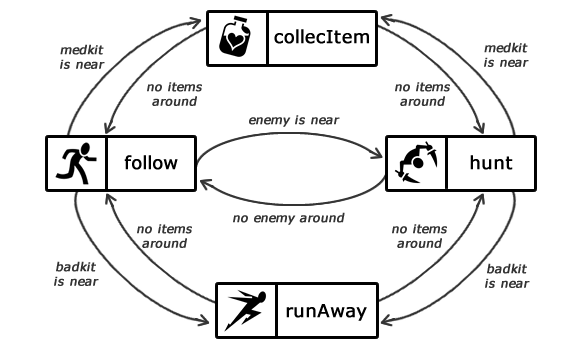
\includegraphics[width=0.85\textwidth]{pics/game.png}
   \end{center}
\end{frame}

\begin{frame}[fragile]
  \transwipe[direction=90]
  \frametitle{Конечные автоматы}
  \begin{center}
     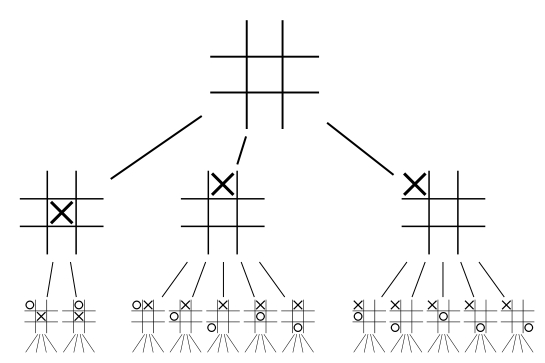
\includegraphics[width=0.85\textwidth]{pics/tictac.jpg}
   \end{center}
\end{frame}

\begin{frame}[fragile]
  \transwipe[direction=90]
  \frametitle{Конечный автомат}
  \textbf{(Детерминированный) конечный автомат} --- $\langle Q, \Sigma, \delta, q_0, F \rangle$
  \begin{itemize}
    \item $Q \neq \varnothing$ --- конечное множество состояний
    \item $\Sigma$ --- Конечный входной алфавит
    \item $\delta$ --- отображение типа $Q \times \Sigma \to Q$
    \begin{itemize}
      \item $\delta(q_i, x) = q_j$
    \end{itemize}
    \item $q_0 \in Q$ --- начальное состояние
    \item $F \subseteq Q$ --- множество конечных состояний
  \end{itemize}

  КА называется \textbf{полным}, если существует переход из каждого состояния по каждому символу алфавита
\begin{itemize}
    \item Обычно добавляют ``дьявольскую'' вершину, она же сток.
\end{itemize}
\end{frame}


\begin{frame}[fragile]
  \transwipe[direction=90]
  \frametitle{Пример конечного автомата}

\[
  Q = \{ q_0, q_1, q_2, q_3\}, \Sigma = \{ 0, 1, -\}, q_0 = q_0, F = \{q_1, q_2\}
\]

\begin{columns}
  \begin{column}{0.4\textwidth}
\[
\begin{array}{rcl}
  \delta (q_0, 0) &=& q_1 \\
  \delta (q_0, 1) &=& q_2 \\
  \delta (q_0, -) &=& q_3 \\
  \delta (q_2, 0) &=& q_2 \\
  \delta (q_2, 1) &=& q_2 \\
  \delta (q_3, 1) &=& q_2
\end{array}
\]
  \end{column}

  \begin{column}{0.6\textwidth}
    \begin{center}
      \begin{tikzpicture}[node distance=2cm, on grid]
        \node[state]           (q_3)                      {$q_3$};
        \node[state,initial]   (q_0) [above left=of q_3]  {$q_0$};
        \node[state,accepting] (q_1) [below left=of q_3]  {$q_1$};
        \node[state,accepting] (q_2) [above right=of q_3] {$q_2$};

        \path[->] (q_0) edge [bend left]  node [above] {$1$}       (q_2)
                        edge              node [left]  {$0$}       (q_1)
                        edge              node [above] {$-$}       (q_3)
                  (q_3) edge              node [above] {$1$}       (q_2)
                  (q_2) edge [loop above] node         {$0$}       ()
                        edge [loop below] node         {$1$}       ();
      \end{tikzpicture}
    \end{center}
  \end{column}
\end{columns}


\end{frame}

\begin{frame}[fragile]
  \transwipe[direction=90]
  \frametitle{Пример полного конечного автомата}
  \begin{center}
    \begin{tikzpicture}[node distance=2cm, on grid]
      \node[state]           (q_3)                      {$q_3$};
      \node[state,initial]   (q_0) [above left=of q_3]  {$q_0$};
      \node[state,accepting] (q_1) [below left=of q_3]  {$q_1$};
      \node[state,accepting] (q_2) [above right=of q_3] {$q_2$};
      \node[state]           (q_d) [below right=of q_3] {$D$};

      \path[->] (q_0) edge [bend left]  node [above] {$1$}       (q_2)
                      edge              node [left]  {$0$}       (q_1)
                      edge              node [above] {$-$}       (q_3)
                (q_3) edge              node [above] {$1$}       (q_2)
                      edge              node [above] {$\ \ 0, -$}(q_d)
                (q_2) edge [loop above] node         {$0$}       ()
                      edge [loop below] node         {$1$}       ()
                      edge [bend left]  node [right] {$-$}       (q_d)
                (q_1) edge              node [above] {$0, 1, -$} (q_d)
                (q_d) edge [loop right] node         {$0, 1, -$} ();
    \end{tikzpicture}
  \end{center}
\end{frame}

\begin{frame}[fragile]
  \transwipe[direction=90]
  \frametitle{Путь в конечном автомате}
  \begin{itemize}
    \item \textbf{Путь} --- кортеж $\langle q_0, e_1, q_1, \dots, e_n, q_n\rangle$
    \begin{itemize}
      \item $n \geq 0$
      \item $\forall i: e_i = \langle q_{i-1}, w_i, q_i \rangle, \text{где } \delta(q_{i-1}, w_i) = q_i$
      \item $q_0$ --- \textbf{начало} пути
      \item $q_n$ --- \textbf{конец} пути
      \item $w_1, w_2, \dots, w_n$ --- \textbf{метка} пути
      \item $n$ --- \textbf{длина} пути
    \end{itemize}
    \item Путь \textbf{успешен}, если $q_0$ --- начальное состояние, а $q_n \in F$
    \item Состояние $q$ \textbf{достижимо} из состояния $p$, если существует путь из состояния $p$ в состояние $q$
  \end{itemize}
\end{frame}

\begin{frame}[fragile]
  \transwipe[direction=90]
  \frametitle{Пример пути}

  \begin{center}
    Успешный путь с меткой $\boldsymbol{-110}$ длины 4
  \end{center}

  \[
    \langle q_0, \langle q_0, -, q_3 \rangle, q_3, \langle q_3, 1, q_2 \rangle, q_2, \langle q_2, 1, q_2 \rangle, q_2, \langle q_2, 0, q_2 \rangle, q_2\rangle
  \]

  \begin{center}
    \begin{tikzpicture}[node distance=2cm, on grid]
      \node[state]           (q_3)                      {$q_3$};
      \node[state,initial]   (q_0) [above left=of q_3]  {$q_0$};
      \node[state,accepting] (q_1) [below left=of q_3]  {$q_1$};
      \node[state,accepting] (q_2) [above right=of q_3] {$q_2$};

      \path[->] (q_0) edge [bend left]  node [above] {$1$}       (q_2)
                      edge              node [left]  {$0$}       (q_1)
                      edge              node [above] {$-$}       (q_3)
                (q_3) edge              node [above] {$1$}       (q_2)
                (q_2) edge [loop above] node         {$0$}       ()
                      edge [loop below] node         {$1$}       ();
    \end{tikzpicture}
  \end{center}
\end{frame}

\begin{frame}[fragile]
  \transwipe[direction=90]
  \frametitle{Такт работы КА (шаг)}
  \begin{itemize}
    \item \textbf{Конфигурация (Мгновенное описание)} КА --- $\langle q, \omega \rangle$, где $q \in Q, \omega \in \Sigma^*$
    \item \textbf{Такт работы} --- бинарное отношение $\vdash$: если $\delta(p , x) = q$ и $\omega \in \Sigma ^*$, то $\langle p , x \omega \rangle \vdash \langle q , \omega \rangle$
    \item Бинарное отношение $\vdash^*$ --- рефлексивное, транзитивное замыкание $\vdash$
  \end{itemize}
\end{frame}

\begin{frame}[fragile]
  \transwipe[direction=90]
  \frametitle{Распознавание слова конечным автоматом}

\begin{center}
  Цепочка $\omega$ \textbf{распознается} КА, если $\exists$ успешный путь с меткой $\omega$
\end{center}

\vspace{20pt}

\begin{center}
  \textbf{Язык, распознаваемый конечным автоматом}: \\ $\{ \omega \in \Sigma^* \mid \exists p$ --- успешный путь с меткой $\omega \}$
\end{center}
\end{frame}

\begin{frame}[fragile]
  \transwipe[direction=90]
  \frametitle{Распознавание слова конечным автоматом: пример}

\[ \{ \dots, -110, -101, -100, -11, -10, -1, 0, 1, 10, 11, 100, 101, 110, \dots\} \]

\begin{center}
  Язык всех целых чисел в двоичной записи
\end{center}

  \begin{center}
    \begin{tikzpicture}[node distance=2cm, on grid]
      \node[state]           (q_3)                      {$q_3$};
      \node[state,initial]   (q_0) [above left=of q_3]  {$q_0$};
      \node[state,accepting] (q_1) [below left=of q_3]  {$q_1$};
      \node[state,accepting] (q_2) [above right=of q_3] {$q_2$};

      \path[->] (q_0) edge [bend left]  node [above] {$1$}       (q_2)
                      edge              node [left]  {$0$}       (q_1)
                      edge              node [above] {$-$}       (q_3)
                (q_3) edge              node [above] {$1$}       (q_2)
                (q_2) edge [loop above] node         {$0$}       ()
                      edge [loop below] node         {$1$}       ();
    \end{tikzpicture}
  \end{center}
\end{frame}


\begin{frame}[fragile]
  \transwipe[direction=90]
  \frametitle{Распознавание слова конечным автоматом}
  \begin{rutheorem}[]
   Рассмотрим конечный автомат  $M = \langle Q , \Sigma , \delta , q_0 , F \rangle$.

   Слово $\omega \in \Sigma ^*$ принадлежит языку $L(M) \iff \exists q \in F: \langle q_0 , \omega \rangle \vdash^* \langle q , \varepsilon \rangle$.
  \end{rutheorem}
\end{frame}

\begin{frame}[fragile]
  \transwipe[direction=90]
  \frametitle{Распознавание слова конечным автоматом}
   Обобщаем функцию перехода:

      \begin{itemize}
        \item $\delta' (q, \varepsilon) = q$
        \item $\delta' (q, x\alpha) = \delta'(\delta(q, x), \alpha) \text{, где } x \in \Sigma, \alpha \in \Sigma^*$
      \end{itemize}

  \begin{rutheorem}[]
     $\text{Цепочка } \omega \textbf{ распознается} \text{ КА } \langle Q, \Sigma, \delta, q_0, F \rangle \iff \exists p \in F : \delta'(q_0, \omega) = p$
  \end{rutheorem}


\begin{center}
     \textbf{Язык, распознаваемый конечным автоматом}: $\{ \omega \in \Sigma^* \mid \exists p \in F : \delta'(q_0, \omega) = p \}$
\end{center}
\end{frame}


\begin{frame}[fragile]
  \transwipe[direction=90]
  \frametitle{Свойство конкатенации строк}
  \begin{rutheorem}[]
    $\langle q_1 , \alpha \rangle \vdash^* \langle q_2 , \varepsilon \rangle, \langle q_2 , \beta \rangle \vdash^* \langle q_3 , \varepsilon \rangle \to \langle q_1 , \alpha \beta \rangle \vdash^* \langle q_3 , \varepsilon \rangle$
  \end{rutheorem}
\end{frame}


\begin{frame}[fragile]
  \transwipe[direction=90]
  \frametitle{Эквивалентность конечных автоматов}
    \begin{center}
      Конечные автоматы $A_1$ и $A_2$ \textbf{эквивалентны}, если распознают один и тот же язык
    \end{center}

    \vspace{20pt}

    \begin{center}
      Как проверить что автоматы эквиваленты?
    \end{center}

\end{frame}

\begin{frame}[fragile]
  \transwipe[direction=90]
  \frametitle{Проверка на эквивалентность автоматов}
  \begin{itemize}
    \item Запустить одновременный обход в ширину двух автоматов
    \item Каждый переход должен приводить в терминальные или нетерминальные вершины в обоих автоматах соответственно
  \end{itemize}
\end{frame}

\begin{frame}[fragile]
  \transwipe[direction=90]
  \frametitle{Минимальный конечный автомат}
   \textbf{Минимальный конечный автомат} --- автомат, имеющий наименьшее число состояний, распознающий тот же язык, что и данный
\end{frame}

\begin{frame}[fragile]
  \transwipe[direction=90]
  \frametitle{Классы эквивалентности}
    \textbf{Отношение эквивалентности} --- рефлексивное, симметричное, транзитивное отношение
    \begin{itemize}
      \item $xRx$
      \item $xRy \iff yRx$
      \item $xRy, yRz \to xRz$
    \end{itemize}

    \begin{rutheorem}
       $\forall R$ --- отношение эквивалентности на множестве $S$

      Можно разбить $S$ на $k$ непересекающихся подмножеств $I_1 \dots I_k$, т.ч. $aRb \iff a, b \in I_j$
    \end{rutheorem}


\begin{center}
      Множества $I_1 \dots I_k$ называются \textbf{классами эквивалентности}
\end{center}
\end{frame}

\begin{frame}[fragile]
  \transwipe[direction=90]
  \frametitle{Эквивалентные состояния}
  \begin{itemize}
    \item $\omega \in \Sigma^*$ \textbf{различает} состояния $q_i$ и $q_j$, если $\delta' (q_i, \omega) = t_1, \delta' (q_j, \omega) = t_2 \to (t_1 \notin F \iff t_2 \in F)$
    \item $q_i$ и $q_j$ \textbf{эквивалентны} $(q_i \sim q_j)$, если $\forall \omega \in \Sigma^*: \delta' (q_i, \omega) = t_1, \delta' (q_j, \omega) = t_2 \to (t_1 \in F \iff t_2 \in F)$
    \begin{itemize}
      \item Является отношением эквивалентности
    \end{itemize}
  \end{itemize}
   \begin{rulemma}
      $\mathcal{A} = \langle Q, \Sigma, \delta, q_0, F \rangle, p_1, p_2, q_1, q_2 \in Q, q_i = \delta(p_i, c)$

      $\omega \in \Sigma^*$ различает $q_1$ и $q_2$. Тогда $c \omega$ различает $p_1$ и $p_2$
   \end{rulemma}

   \begin{ruproof}
     $\delta' (p_i, c \omega) = \delta' (\delta (p_i, c), \omega) = \delta' (q_i, \omega) = t_i$
   \end{ruproof}
\end{frame}

\begin{frame}[fragile]
  \transwipe[direction=90]
  \frametitle{Алгоритм минимизации КА}
    TLDR: разбиваем состояния на классы эквивалентности, которые делаем новыми состояниями

\end{frame}

\begin{frame}[fragile]
  \transwipe[direction=90]
  \frametitle{Алгоритм минимизации КА}

     $Q$ --- очередь

     \vspace{10pt}

     $marked$ --- таблица размером $n \times n$ (n --- количество состояний КА).

     \vspace{10pt}

      Помечаем в таблице пары неэквивалентных состояний и кладем их в очередь

\end{frame}

\begin{frame}[fragile]
  \transwipe[direction=90]
  \frametitle{Алгоритм минимизации КА}
    \begin{itemize}
      \item Если автомат не полный --- дополнить дьявольской вершиной
      \item Строим отображение $\delta^{-1}$ --- обратные ребра
      \item Находим все достижимые из стартового состояния
      \item Добавляем в $Q$ и отмечаем в $marked$ пары состояний, различимые $\varepsilon$
      \item Можем пометить пару $(u, v)$, если $\exists c \in \Sigma :  (\delta(u, c), \delta(v, c)) помечена$. Для этого, пока $Q \neq \varnothing$:
      \begin{itemize}
        \item Извлекаем $(u, v)$ из $Q$
        \item $\forall c \in \Sigma$ перебираем $(\delta^{-1}(u, c), \delta^{-1}(v, c))$ --- если пара не помечена, помечаем и кладем в очередь
      \end{itemize}
      \item В момент опустошения $Q$ непомеченные пары являются эквивалентными
      \item За проход по таблице выделяем классы эквивалентности
      \item За проход по таблице формируем новые состояния и переходы
    \end{itemize}

\end{frame}

\begin{frame}[fragile]
  \transwipe[direction=90]
  \frametitle{Алгоритм минимизации КА}
    \begin{itemize}
      \item Стартовое состояние --- класс эквивалентности, которому принадлежит стартовое состояние исходного КА
      \item Конечные состояния --- классы эквивалентности, которым принадлежат конечные состояния исходного КА
    \end{itemize}

\end{frame}

\begin{frame}[fragile]
  \transwipe[direction=90]
  \frametitle{Алгоритм минимизации КА: корректность}
    \begin{itemize}
      \item Пусть в результате применения алгоритма к КА $A$ получили КА $A_{min}$. Покажем, что этот автомат минимальный и единственный с точностью до изоморфизма
      \item Пусть $\exists A' : A'$ и $A$ эквивалентны, но количество состояний $A'$ меньше, чем у $A_{min}$
      \item Стартовые состояния $s \in A_{min}$ и $s' \in A'$ эквивалентны (КА допускают один язык)
      \item $\sphericalangle \alpha = a_1 a_2 \dots a_k, a_i \in \Sigma: \langle s, \alpha \rangle \vdash^* \langle u, \varepsilon \rangle; \langle s', \alpha \rangle \vdash^* \langle u', \varepsilon \rangle$
      \item $\sphericalangle \langle s, a_1 \rangle \vdash^* \langle l, \varepsilon \rangle; \langle s', a_1 \rangle \vdash^* \langle l', \varepsilon \rangle$. $s, s'$ эквивалентны $\to l, l'$ эквивалентны
      \item Аналогично для всех $a_i \Mapsto u, u'$ эквивалентны
      \item $\Mapsto \forall q$ --- состояние $A_{min} \exists q'$ --- эквивалентное состояние $A'$
      \item Состояний $A'$ меньше, чем состояний $A_{min} \to$ 2 состояниям $A_{min}$ соответствует 1 состояние $A' \to$ они эквивалентны. Но по построению $A_{min}$ в нем не может быть эквивалентных состояний. Противоречие
    \end{itemize}

\end{frame}


\begin{frame}[fragile]
  \transwipe[direction=90]
  \frametitle{Недетерминированный КА}
 \textbf{Недетерминированный конечный автомат} --- $\langle Q, \Sigma, \delta, q_0, F \rangle$
  \begin{itemize}
    \item $Q \neq \varnothing$ --- конечное множество состояний
    \item $\Sigma$ --- Конечный входной алфавит
    \item $\delta$ --- отображение типа $Q \times \Sigma \rightarrow 2^Q$
    \begin{itemize}
      \item $\delta(q_i, x) = \{ q_{j_0}, \dots, q_{j_k} \}$
    \end{itemize}
    \item $q_0 \in Q$ --- начальное состояние
    \item $F \subseteq Q$ --- множество конечных состояний
  \end{itemize}

\end{frame}

\begin{frame}[fragile]
  \transwipe[direction=90]
  \frametitle{Недетерминированный КА: пример}

\begin{columns}
  \begin{column}{0.25\textwidth}
\[
  \begin{array}{rcl}
    \delta (q_0, \text{а}) &=& q_0 \\
     &\dots&  \\
    \delta (q_0, \text{к}) &=& q_0 \\
    &\dots&  \\
    \delta (q_0, \text{я}) &=& q_0 \\

    \delta (q_0, \text{к}) &=& q_1 \\

    & & \\

    \delta (q_1, \text{о}) &=& q_2 \\

    & & \\

    \delta (q_2, \text{т}) &=& q_3 \\

    & & \\

    \delta (q_3, \text{а}) &=& q_3 \\
    &\dots&  \\
   \delta (q_3, \text{я}) &=& q_3 \\
  \end{array}
\]
  \end{column}

  \begin{column}{0.75\textwidth}
      \begin{center}
        \begin{tikzpicture}[node distance=2cm, on grid]
          \node[state,initial]   (q_0)                 {$q_0$};
          \node[state]           (q_1) [right =of q_0] {$q_1$};
          \node[state]           (q_2) [right =of q_1] {$q_2$};
          \node[state,accepting] (q_3) [right =of q_2] {$q_3$};

          \path[->] (q_0) edge node [above] {к} (q_1)
                          edge [loop above] node [above] {a\dots к\dots я} ()
                    (q_1) edge node [above] {о} (q_2)
                    (q_2) edge node [above] {т} (q_3)
                    (q_3) edge [loop above] node [above] {a\dots я} ();
        \end{tikzpicture}
      \end{center}
  \end{column}
\end{columns}
\end{frame}

\begin{frame}[fragile]
  \transwipe[direction=90]
  \frametitle{Распознавание слова НКА}
  \begin{itemize}
    \item \textbf{Конфигурация (Мгновенное описание)} КА --- $\langle q, \omega \rangle$, где $q \in Q, \omega \in \Sigma^*$
    \item \textbf{Такт работы} --- бинарное отношение $\vdash$: если $q \in \delta(p, x)$ и $\omega \in \Sigma ^*$, то $\langle p , x \omega \rangle \vdash \langle q , \omega \rangle$
    \item Бинарное отношение $\vdash^*$ --- рефлексивное, транзитивное замыкание $\vdash$
    \item НКА \textbf{допускает} слово $\alpha$, если $\exists t \in F : \langle s, \alpha \rangle \vdash^* \langle t, \varepsilon \rangle$
    \item \textbf{Язык НКА} $L(A) = \{ \omega \in \Sigma^* \mid \exists t \in F : \langle s, \omega \rangle \vdash^* \langle t, \varepsilon \rangle \}$
  \end{itemize}
  \begin{itemize}
    \item ДКА --- частный случай НКА
  \end{itemize}
\end{frame}

\begin{frame}[fragile]
  \transwipe[direction=90]
  \frametitle{Недетерминированный КА: пример}

      \begin{center}
        \begin{tikzpicture}[node distance=2cm, on grid]
          \node[state,initial]   (q_0)                 {$q_0$};
          \node[state]           (q_1) [right =of q_0] {$q_1$};
          \node[state]           (q_2) [right =of q_1] {$q_2$};
          \node[state,accepting] (q_3) [right =of q_2] {$q_3$};

          \path[->] (q_0) edge node [above] {к} (q_1)
                          edge [loop above] node [above] {a\dots к\dots я} ()
                    (q_1) edge node [above] {о} (q_2)
                    (q_2) edge node [above] {т} (q_3)
                    (q_3) edge [loop above] node [above] {a\dots я} ();
        \end{tikzpicture}
      \end{center}

\vspace{20pt}

  \begin{center}
    \{\textbf{кот}, с\textbf{кот}, \textbf{кот}лета, мя\textbf{кот}ь, антре\textbf{кот}\dots \}
  \end{center}
\end{frame}

\begin{frame}[fragile]
  \transwipe[direction=90]
  \frametitle{Алгоритм, определяющий допустимость слова}

\[
\begin{array}{rcl}
  R(\alpha)      &=& \{ p \mid \langle q_0, \alpha \rangle \vdash^* \langle p, \varepsilon \rangle\} \\
  & & \\
  R(\varepsilon) &=& \{q_0\} \\
  R(\alpha c)    &=& \{q \mid q \in \delta (p, c), p \in R(\alpha)\}
\end{array}
\]

\vspace{20pt}

\begin{center}
  НКА допускает слово $\alpha \iff \exists t \in F : t \in R(\alpha) $
\end{center}

\end{frame}

\begin{frame}[fragile]
  \transwipe[direction=90]
  \frametitle{Построение ДКА по НКА}
  \begin{itemize}
    \item Помещаем в $Queue$ множество $\{ q_0 \}$
    \item Пока очередь не пуста, выполняем:
    \begin{itemize}
      \item $q = Queue.pop()$
      \item Строим множество $q' = \{t = \delta (s, c) \mid s \in q, c \in \Sigma\}$. Если $q' \notin Queue$, добавить его в очередь. Каждое такое множество --- новая вершина ДКА; добавляем переходы по соответствующим символам
      \item Если во множестве есть хотя бы одна вершина, являющаяся терминальной в данном НКА, то соответствующая вершина ДКА будет конечной
    \end{itemize}
  \item Результат: $\langle \Sigma, Q_d, q_{d_0} \in Q_d, F_d \subset Q_d, \delta_d: Q_d \times \Sigma \rightarrow {Q_d} \rangle$
  \begin{itemize}
    \item $Q_d = \{q_d \mid q_d \subset 2^Q \}$
    \item $q_{d_0} = \{q_0\}$
    \item $F_d = \{q \in Q_d \mid \exists p \in F : p \in q\}$
    \item $\delta_d(q, c) = \{ \delta(a, c) \mid a \in q \}$
  \end{itemize}
  \end{itemize}
\end{frame}

\begin{frame}[fragile]
  \transwipe[direction=90]
  \frametitle{Детерминизация НКА: пример}
    \begin{center}
      \begin{tikzpicture}[node distance=2cm, on grid]
        \node[state,initial]   (q_0)                 {$1$};
        \node[state,accepting] (q_1) [right =of q_0] {$2$};

        \path[->] (q_0) edge [bend left]  node [above] {a}   (q_1)
                        edge [loop above] node [above] {a,b} ()
                  (q_1) edge [bend left]  node [below] {b}   (q_0)
                        edge [loop above] node [above] {b}   ();
      \end{tikzpicture}
    \end{center}

    \begin{center}
      \begin{tikzpicture}[node distance=2cm, on grid]
        \node[state,initial]   (q_0)                 {$1$};
        \node[state,accepting] (q_1) [right =of q_0] {$1, 2$};

        \path[->] (q_0) edge              node [above] {a}   (q_1)
                        edge [loop above] node [above] {b}   ()
                  (q_1) edge [loop above] node [above] {a,b} ();
      \end{tikzpicture}
    \end{center}

\end{frame}



\begin{frame}[fragile]
  \transwipe[direction=90]
  \frametitle{Эквивалентность языков, распознаваемых ДКА и НКА}
  \begin{rutheorem}
  ДКА и НКА распознают один и тот же класс языков
  \end{rutheorem}
  \begin{proof}
  $\Rightarrow: $ очевидно

  $\Leftarrow: $ Рассмотрим произвольный НКА и покажем, что алгоритм строит по нему эквивалентный ДКА.

  $\forall q \in q_d, \forall c \in \Sigma, \forall p \in \delta(q, c): p \in \delta_d (q_d, c)$

  Рассмотрим $\langle q_0, w_1 w_2 \dots w_m \rangle \vdash \langle u_1, w_2 \dots w_m\rangle  \vdash^* \langle u_m, \varepsilon \rangle, u_m \in F $

  $\forall i: u_i \in u_{d_i}, $ где $(q_{d_0}, w_1 w_2 \dots w_m) \vdash (u_{d_1}, w_2 \dots w_m) \vdash^* (u_{d_m}, \varepsilon)$

  $\Mapsto u_m \in u_{d_m}$
  \end{proof}
\end{frame}



\begin{frame}[fragile]
  \transwipe[direction=90]
  \frametitle{Распознание слова НКА}
  \begin{myauto}[2.5]
    \node[state,accepting] (q_2)                 {C};
    \node[state,initial]   (q_0)  [left=of q_2]  {A};
    \node[state,accepting] (q_1)  [above=of q_2] {B};
    \node[state]           (q_3)  [below=of q_2] {D};
    \node[state,accepting] (q_4)  [right=of q_1] {E};
    \node[state]           (q_5)  [right=of q_2] {F};

    \path[->] (q_0) edge                node [above] {$a$} (q_1)
                    edge                node [above] {$a$} (q_2)
                    edge                node [above] {$a$} (q_3)
              (q_1) edge                node [above] {$b$} (q_4)
              (q_3) edge [bend left=15] node [above] {$b$} (q_5)
              (q_4) edge [loop below]   node [below] {$b$} ()
              (q_5) edge [bend left=15] node [below] {$a$} (q_3)
              (q_5) edge                node [above] {$a$} (q_2)
              ;
  \end{myauto}


  \begin{center}
    Слово распознается за $O(|\omega| \sum\limits_{t \in Q} \sum\limits_{c \in \Sigma} |\delta(t, c)|)$
  \end{center}
\end{frame}



\begin{frame}[fragile]
  \transwipe[direction=90]
  \frametitle{Произведение автоматов}
   $A_1 = \langle \Sigma_1, Q_1, q_{1_0}, \delta_1, F_1 \rangle$ и $A_2 = \langle \Sigma_2, Q_2, q_{2_0}, \delta_2, F_2 \rangle$ --- КА

   \vfill

  \textbf{Произведением} автоматов назовем $A = \langle \Sigma, Q, q_0, \delta, F \rangle$, где

  \vfill

  \begin{itemize}
    \item $\Sigma = \Sigma_1 \cup \Sigma_2$
    \item $Q = Q_1 \times Q_2$
    \item $q_0 = (q_{1_0}, q_{2_0})$
    \item $F \subseteq Q$
    \begin{itemize}
      \item $F = F_1 \times F_2$ --- распознает \textbf{пересечение} языков
      \item $F = (F_1 \times Q_2) \cup (Q_1 \times F_2)$ --- распознает \textbf{объединение} языков
      \item $F = F_1 \times (Q_2 \setminus F_2)$ --- распознает \textbf{разность} языков
    \end{itemize}
    \item $\delta((q_1, q_2), c) = (\delta_1(q_1, c), \delta_2(q_2, c))$
  \end{itemize}

  \vfill

  Интуиция: ищем пути в двух автоматах одновременно
\end{frame}


\begin{frame}[fragile]
  \transwipe[direction=90]
  \frametitle{Произведение автоматов: пример}
  \begin{columns}
    \begin{column}{0.4\textwidth}
      \begin{myauto}[2]
        \node[state,initial]   (q_0)                {A};
        \node[state,accepting] (q_1) [right of=q_0] {B};

        \path[->] (q_0) edge [loop above] node [above] {$0$}    ()
                        edge              node [above] {$1$}    (q_1)
                  (q_1) edge [loop above] node [above] {$0, 1$} ();
      \end{myauto}
    \end{column}

    \begin{column}{0.6\textwidth}
      \begin{myauto}[2]
        \node[state,initial]   (p_0)                {X};
        \node[state]           (p_1) [right of=q_0] {Y};
        \node[state,accepting] (p_2) [right of=q_1] {Z};

        \path[->] (p_0) edge [loop above] node [above] {$1$}    ()
                        edge              node [above] {$0$}    (p_1)
                  (p_1) edge [loop above] node [above] {$0$}    ()
                        edge              node [above] {$1$}    (p_2)
                  (p_2) edge [loop above] node [above] {$0, 1$} ()
                  ;
      \end{myauto}
    \end{column}
  \end{columns}

  \begin{myauto}[2.3]
    \node[state,initial]   (s_00)                 {A,X};
    \node[state]           (s_01) [right of=s_00] {A,Y};
    \node[state,thin]      (s_02) [right of=s_01] {A,Z};
    \node[state]           (s_10) [below of=s_00] {B,X};
    \node[state]           (s_11) [below of=s_01] {B,Y};
    \node[state]           (s_12) [below of=s_02] {B,Z};

    \path[->] (s_00) edge                    node [above] {$0$}   (s_01)
                     edge                    node [left]  {$1$}   (s_10)
              (s_01) edge [loop above]       node [above] {$0$}   ()
                     edge                    node [right] {$1$}   (s_12)
              (s_02) edge [loop above, thin] node [above] {$0$}   ()
                     edge [thin]             node [right] {$1$}   (s_12)
              (s_10) edge [loop below]       node [below] {$1$}   ()
                     edge                    node [above] {$0$}   (s_11)
              (s_11) edge [loop below]       node [below] {$0$}   ()
                     edge                    node [above] {$1$}   (s_12)
              (s_12) edge [loop right]       node [right] {$0,1$} (s_12)
              ;
  \end{myauto}
\end{frame}

\begin{frame}[fragile]
  \transwipe[direction=90]
  \frametitle{Пересечение языков}
  \begin{columns}
    \begin{column}{0.4\textwidth}
      \begin{myauto}[2]
        \node[state,initial]   (q_0)                {A};
        \node[state,accepting] (q_1) [right of=q_0] {B};

        \path[->] (q_0) edge [loop above] node [above] {$0$}    ()
                        edge              node [above] {$1$}    (q_1)
                  (q_1) edge [loop above] node [above] {$0, 1$} ();
      \end{myauto}
    \end{column}

    \begin{column}{0.6\textwidth}
      \begin{myauto}[2]
        \node[state,initial]   (p_0)                {X};
        \node[state]           (p_1) [right of=q_0] {Y};
        \node[state,accepting] (p_2) [right of=q_1] {Z};

        \path[->] (p_0) edge [loop above] node [above] {$1$}    ()
                        edge              node [above] {$0$}    (p_1)
                  (p_1) edge [loop above] node [above] {$0$}    ()
                        edge              node [above] {$1$}    (p_2)
                  (p_2) edge [loop above] node [above] {$0, 1$} ()
                  ;
      \end{myauto}
    \end{column}
  \end{columns}

  \begin{myauto}[2.3]
    \node[state,initial]   (s_00)                 {A,X};
    \node[state]           (s_01) [right of=s_00] {A,Y};
    \node[state,thin]      (s_02) [right of=s_01] {A,Z};
    \node[state]           (s_10) [below of=s_00] {B,X};
    \node[state]           (s_11) [below of=s_01] {B,Y};
    \node[state,accepting] (s_12) [below of=s_02] {B,Z};

    \path[->] (s_00) edge                    node [above] {$0$}   (s_01)
                     edge                    node [left]  {$1$}   (s_10)
              (s_01) edge [loop above]       node [above] {$0$}   ()
                     edge                    node [right] {$1$}   (s_12)
              (s_02) edge [loop above, thin] node [above] {$0$}   ()
                     edge [thin]             node [right] {$1$}   (s_12)
              (s_10) edge [loop below]       node [below] {$1$}   ()
                     edge                    node [above] {$0$}   (s_11)
              (s_11) edge [loop below]       node [below] {$0$}   ()
                     edge                    node [above] {$1$}   (s_12)
              (s_12) edge [loop right]       node [right] {$0,1$} (s_12)
              ;
  \end{myauto}
\end{frame}

\begin{frame}[fragile]
  \transwipe[direction=90]
  \frametitle{Объединение языков}
  \begin{columns}
    \begin{column}{0.4\textwidth}
      \begin{myauto}[2]
        \node[state,initial]   (q_0)                {A};
        \node[state,accepting] (q_1) [right of=q_0] {B};

        \path[->] (q_0) edge [loop above] node [above] {$0$}    ()
                        edge              node [above] {$1$}    (q_1)
                  (q_1) edge [loop above] node [above] {$0, 1$} ();
      \end{myauto}
    \end{column}

    \begin{column}{0.6\textwidth}
      \begin{myauto}[2]
        \node[state,initial]   (p_0)                {X};
        \node[state]           (p_1) [right of=q_0] {Y};
        \node[state,accepting] (p_2) [right of=q_1] {Z};

        \path[->] (p_0) edge [loop above] node [above] {$1$}    ()
                        edge              node [above] {$0$}    (p_1)
                  (p_1) edge [loop above] node [above] {$0$}    ()
                        edge              node [above] {$1$}    (p_2)
                  (p_2) edge [loop above] node [above] {$0, 1$} ()
                  ;
      \end{myauto}
    \end{column}
  \end{columns}

  \begin{myauto}[2.3]
    \node[state,initial]        (s_00)                 {A,X};
    \node[state]                (s_01) [right of=s_00] {A,Y};
    \node[state,thin,accepting] (s_02) [right of=s_01] {A,Z};
    \node[state,accepting]      (s_10) [below of=s_00] {B,X};
    \node[state,accepting]      (s_11) [below of=s_01] {B,Y};
    \node[state,accepting]      (s_12) [below of=s_02] {B,Z};

    \path[->] (s_00) edge                    node [above] {$0$}   (s_01)
                     edge                    node [left]  {$1$}   (s_10)
              (s_01) edge [loop above]       node [above] {$0$}   ()
                     edge                    node [right] {$1$}   (s_12)
              (s_02) edge [loop above, thin] node [above] {$0$}   ()
                     edge [thin]             node [right] {$1$}   (s_12)
              (s_10) edge [loop below]       node [below] {$1$}   ()
                     edge                    node [above] {$0$}   (s_11)
              (s_11) edge [loop below]       node [below] {$0$}   ()
                     edge                    node [above] {$1$}   (s_12)
              (s_12) edge [loop right]       node [right] {$0,1$} (s_12)
              ;
  \end{myauto}
\end{frame}

\begin{frame}[fragile]
  \transwipe[direction=90]
  \frametitle{Разность языков}
  \begin{columns}
    \begin{column}{0.4\textwidth}
      \begin{myauto}[2]
        \node[state,initial]   (q_0)                {A};
        \node[state,accepting] (q_1) [right of=q_0] {B};

        \path[->] (q_0) edge [loop above] node [above] {$0$}    ()
                        edge              node [above] {$1$}    (q_1)
                  (q_1) edge [loop above] node [above] {$0, 1$} ();
      \end{myauto}
    \end{column}

    \begin{column}{0.6\textwidth}
      \begin{myauto}[2]
        \node[state,initial]   (p_0)                {X};
        \node[state]           (p_1) [right of=q_0] {Y};
        \node[state,accepting] (p_2) [right of=q_1] {Z};

        \path[->] (p_0) edge [loop above] node [above] {$1$}    ()
                        edge              node [above] {$0$}    (p_1)
                  (p_1) edge [loop above] node [above] {$0$}    ()
                        edge              node [above] {$1$}    (p_2)
                  (p_2) edge [loop above] node [above] {$0, 1$} ()
                  ;
      \end{myauto}
    \end{column}
  \end{columns}

  \begin{myauto}[2.3]
    \node[state,initial]   (s_00)                 {A,X};
    \node[state]           (s_01) [right of=s_00] {A,Y};
    \node[state,thin]      (s_02) [right of=s_01] {A,Z};
    \node[state,accepting] (s_10) [below of=s_00] {B,X};
    \node[state,accepting] (s_11) [below of=s_01] {B,Y};
    \node[state]           (s_12) [below of=s_02] {B,Z};

    \path[->] (s_00) edge                    node [above] {$0$}   (s_01)
                     edge                    node [left]  {$1$}   (s_10)
              (s_01) edge [loop above]       node [above] {$0$}   ()
                     edge                    node [right] {$1$}   (s_12)
              (s_02) edge [loop above, thin] node [above] {$0$}   ()
                     edge [thin]             node [right] {$1$}   (s_12)
              (s_10) edge [loop below]       node [below] {$1$}   ()
                     edge                    node [above] {$0$}   (s_11)
              (s_11) edge [loop below]       node [below] {$0$}   ()
                     edge                    node [above] {$1$}   (s_12)
              (s_12) edge [loop right]       node [right] {$0,1$} (s_12)
              ;
  \end{myauto}
\end{frame}

\begin{frame}[fragile]
  \transwipe[direction=90]
  \frametitle{Замкнутость автоматных языков относительно операций}
  Автоматные языки замкнуты относительно операций:

  \begin{itemize}
    \item Объединения
    \item Пересечения
    \item Разности
    \item Дополнения
    \begin{itemize}
      \item $\overline{X} = \Sigma^* \setminus X$
    \end{itemize}
  \end{itemize}
\end{frame}

\begin{frame}[fragile]
  \transwipe[direction=90]
  \frametitle{Регулярное множество (регулярный язык)}
    \textbf{Регулярное множество} в алфавите $\Sigma$ определяется итеративно:

    \begin{itemize}
      \item $\varnothing $ --- регулярное множество в алфавите $\Sigma$
      \item $\{a\}$  --- регулярное множество в алфавите $\Sigma$ для каждого $a \in \Sigma$
      \item $\{\varepsilon\}$  --- регулярное множество в алфавите $\Sigma$
      \item Если $P$ и $Q$ --- регулярные множества в алфавите $\Sigma$, то регулярны
      \begin{itemize}
        \item $P \cup Q$ \hfill (объединение)
        \item $PQ = \{ pq \mid p \in P, q \in Q\}$ \hfill (конкатенация)
        \item $P^* = \{\varepsilon\} \cup P \cup PP \cup PPP \cup \dots $ \hfill (итерация)
      \end{itemize}
      \item Ничто другое не является регулярным множеством в алфавите $\Sigma$
      \item Множество всех регулярных языков обозначим $\mathbb{R}$
    \end{itemize}
\end{frame}

\begin{frame}[fragile]
  \transwipe[direction=90]
  \frametitle{Примеры регулярных языков}
  \begin{itemize}
   \item Все конечные языки
    \begin{itemize}
     \item $\{-2 147 483 648, -2 147 483 647, \dots,  2 147 483 647\}$ --- все 32-разрядные целые числа
    \end{itemize}
    \item $L_a = \{a^k \mid k - odd \} $
    \item $L_b = \{b^l \mid l - even \} $
    \item $L_{ab} = \{a^k b^l \mid k - odd, l - even\} =  L_a L_b$
    \item $L = \{a^*\} = L_a^*$
  \end{itemize}


\end{frame}

\begin{frame}[fragile]
  \transwipe[direction=90]
  \frametitle{Регулярное выражение}
    \textbf{Регулярное выражение} --- способ записи регулярного множества


    \begin{itemize}
      \item $\varnothing $ --- обозначает $\varnothing$
      \item $a$  --- обозначает $\{a\}$
      \item $\varepsilon$  --- обозначает $\{\varepsilon\}$
      \item Если $p$ и $q$ обозначают $P$ и $Q$, то:
      \begin{itemize}
        \item $p \mid q$ обозначает $P \cup Q$
        \item $pq$ обозначает $PQ$
        \item $p^*$ обозначает $P^*$
      \end{itemize}
    \end{itemize}
\end{frame}

\begin{frame}[fragile]
  \transwipe[direction=90]
  \frametitle{Примеры регулярных выражений}
  \begin{itemize}
    \item $-2 147 483 648 \mid -2 147 483 647 \mid \dots \mid  2 147 483 647$ --- все 32-разрядные целые числа
    \item $a(aa)^*: L_a = \{a^k \mid k - odd \} $
    \item $(bb)^*: L_b = \{b^l \mid l - even \} $
    \item $a(aa)^* (bb)^* :  L_{ab} = \{a^k b^l \mid k - odd, l - even\} =  L_a L_b$
    \item $a^* : L = \{a^*\} = L_a^*$
  \end{itemize}
\end{frame}


\begin{frame}[fragile]
  \transwipe[direction=90]
  \frametitle{Замкнутость регулярных языков относительно операций}
  Регулярные языки замкнуты ($A \in \mathbb{R}, B \in \mathbb{R} \Rightarrow A \diamond B \in \mathbb{R}$) относительно операций:
  \begin{itemize}
    \item Конкатенации $ (L_1 L_2) $, объединения $ (L_1 \cup L_2) $, итерации $ (L^*) $
    \item Пересечения $ (L_1 \cap L_2) $, дополнения $ (\neg L)$, разности $ (L_1 \setminus L_2) $
    \item Обращения $(L_{rev} = \{\omega^R = a_m a_{m-1} \dots a_1 \mid a_1 a_2 \dots a_m = \omega \in L \})$
    \item Гомоморфизма цепочек $\phi$
    \begin{itemize}
      \item $\phi(\varepsilon) = \varepsilon$
      \item $\phi(\alpha \beta) = \phi(\alpha) \phi(\beta)$
    \end{itemize}
    \item Обратного гомоморфизма цепочек
  \end{itemize}
\end{frame}


\begin{frame}[fragile]
  \transwipe[direction=90]
  \frametitle{Теорема Клини}
  \begin{rutheorem}
   Классы автоматных и регулярных языков \emph{эквивалентны}
  \end{rutheorem}
\end{frame}


\begin{frame}[fragile]
  \transwipe[direction=90]
  \frametitle{НКА с $\varepsilon$-переходами: почему бы и нет?}
  \[ \delta: Q \times (\Sigma \cup \varepsilon) \to 2^Q \]


  \begin{myauto}
    \node[state,initial]   (q_0)                {A};
    \node[state]           (q_1) [right of=q_0] {B};
    \node[state,accepting] (q_2) [right of=q_1] {C};

    \path[->] (q_0) edge [loop above]   node [above] {$1$}           ()
                    edge [bend left=15] node [above] {$0$}           (q_1)
              (q_1) edge [bend left=15] node [above] {$0$}           (q_2)
                    edge [bend left=15] node [below] {$\varepsilon$} (q_0)
              (q_2) edge [bend left=15] node [below] {$1$}           (q_1)
                    edge [loop above]   node [above] {$0$}           ()
              ;
  \end{myauto}

 \begin{center}
    Ничего не поломалось?
 \end{center}
\end{frame}

\begin{frame}[fragile]
  \transwipe[direction=90]
  \frametitle{Эквивалентность НКА с $\varepsilon$-переходами и НКА без $\varepsilon$-переходов }
  \begin{itemize}
    \item НКА без $\varepsilon$-переходов --- частный случай НКА с $\varepsilon$-переходами
    \item В обратную сторону --- можно построить $\varepsilon$-замыкание
    \begin{itemize}
      \item Транзитивное замыкание: для каждого подграфа, состоящего только из $\varepsilon$-переходов, делаем $\varepsilon$-замыкание
      \item Добавление терминальных состояний: для $\varepsilon$-перехода из состояния $u$ в $v$, где $v$ --- терминальное, добавляем $u$ в терминальные
      \item Добавление ребер: $\forall u, v, c, w: \delta(u,\varepsilon)=v, \delta(v,c)=w$, добавим переход $\delta(u,c)=w$
      \item Устранение $\varepsilon$-переходов
    \end{itemize}
  \end{itemize}
\end{frame}

\begin{frame}
  \transwipe[direction=90]
  \frametitle{$\varepsilon$-замыкание}
  \begin{myauto}
    \node[state,initial]   (q_0)                {A};
    \node[state]           (q_1) [right of=q_0] {B};
    \node[state,accepting] (q_2) [right of=q_1] {C};

    \path[->] (q_0) edge [loop above]   node [above] {$1$}           ()
                    edge [bend left=15] node [above] {$\varepsilon$} (q_1)
              (q_1) edge [bend left=15] node [below] {$0$}           (q_0)
                    edge [bend left=15] node [above] {$\varepsilon$} (q_2)
              (q_2) edge [bend left=15] node [below] {$\varepsilon$} (q_1)
                    edge [loop above]   node [above] {$\varepsilon$} ()
              ;
  \end{myauto}

  \begin{columns}
    \begin{column}{0.5\textwidth}
      \begin{myauto}
        \node[state,initial]   (q_0)                {A};
        \node[state,accepting] (q_1) [right of=q_0] {BC};

        \path[->] (q_0) edge [loop above]   node [above] {$1$}           ()
                        edge [bend left=15] node [above] {$\varepsilon$} (q_1)
                  (q_1) edge [bend left=15] node [below] {$0$}           (q_0)
                  ;
      \end{myauto}
    \end{column}

    \begin{column}{0.5\textwidth}
      \begin{myauto}
        \node[state,initial,accepting]   (q_0)                {A};
        \node[state,accepting]           (q_1) [right of=q_0] {BC};

        \path[->] (q_0) edge [loop above]   node [above] {$1$}           ()
                        edge [bend left=15] node [above] {$\varepsilon$} (q_1)
                  (q_1) edge [bend left=15] node [below] {$0$}           (q_0)
                  ;
      \end{myauto}
    \end{column}
  \end{columns}

  \begin{myauto}
    \node[state,initial,accepting] (q_0) {A};

    \path[->] (q_0) edge [loop above]   node [above] {$0,1$} ()
              ;
  \end{myauto}
 \end{frame}

\begin{frame}
  \transwipe[direction=90]
  \frametitle{Теорема Клини: доказательство $\Leftarrow$}

  \begin{rutheorem}
   Классы автоматных и регулярных языков \emph{эквивалентны}
  \end{rutheorem}

  \begin{proof}
    $\Leftarrow:$ Построим по регулярному выражению КА (НКА с $\varepsilon$-переходами)
  \end{proof}
\end{frame}

\begin{frame}
  \transwipe[direction=90]
  \frametitle{Построение КА по РВ: $\varepsilon$}
    \begin{center}
      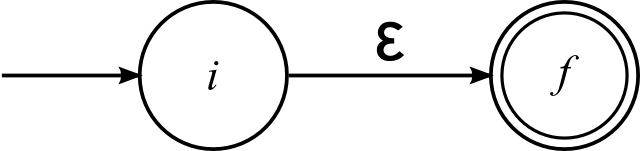
\includegraphics[width=0.40\textwidth]{pics/epsilon.png}
    \end{center}
\end{frame}

\begin{frame}
  \transwipe[direction=90]
  \frametitle{Построение КА по РВ: символ}
    \begin{center}
      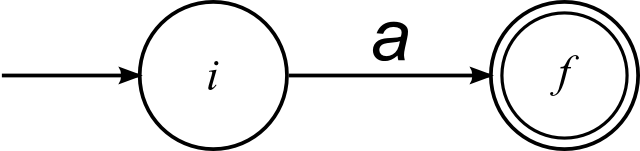
\includegraphics[width=0.40\textwidth]{pics/terminal.png}
    \end{center}
\end{frame}

\begin{frame}
  \transwipe[direction=90]
  \frametitle{Построение КА по РВ: объединение $p \mid q$}
    \begin{center}
      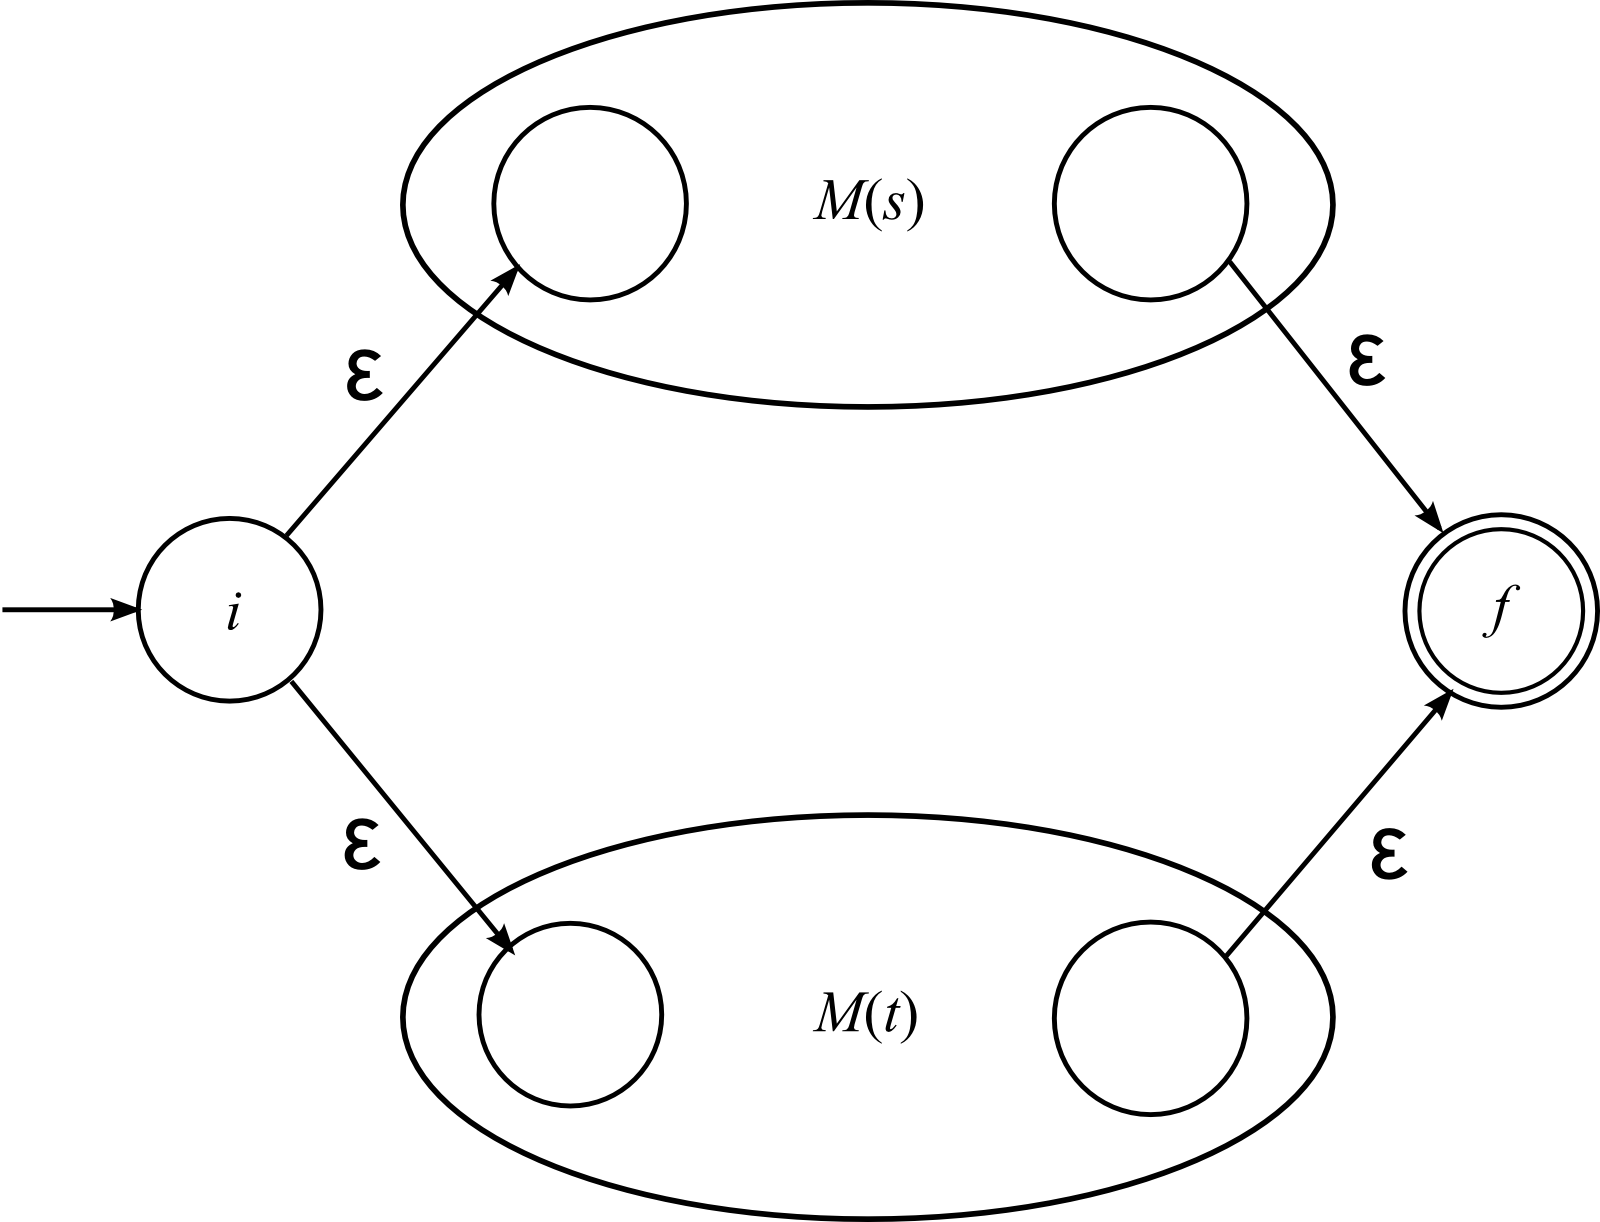
\includegraphics[width=0.80\textwidth]{pics/union.png}
    \end{center}
\end{frame}

\begin{frame}
  \transwipe[direction=90]
  \frametitle{Построение КА по РВ: конкатенация $p q$}
    \begin{center}
      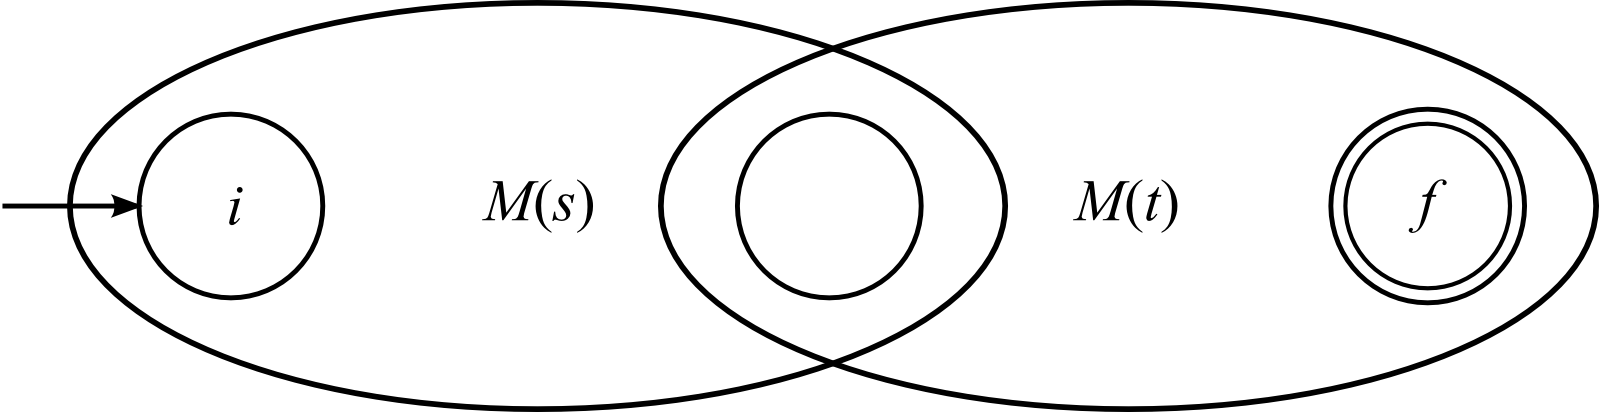
\includegraphics[width=0.80\textwidth]{pics/concat.png}
    \end{center}
\end{frame}

\begin{frame}
  \transwipe[direction=90]
  \frametitle{Построение КА по РВ: итерация $p^*$}
    \begin{center}
      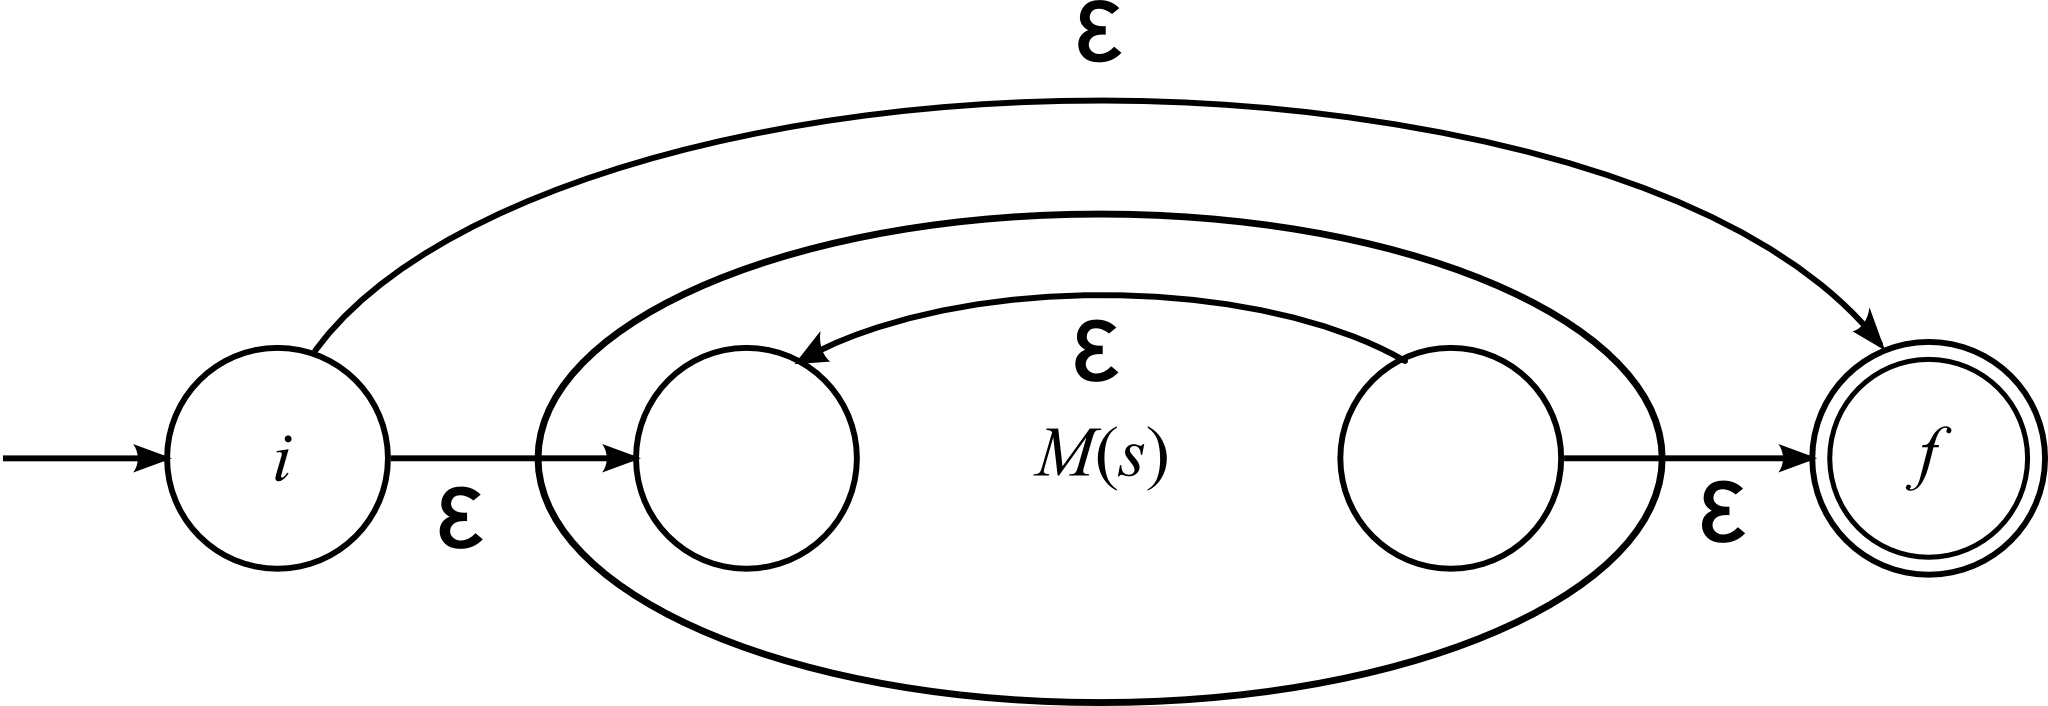
\includegraphics[width=0.80\textwidth]{pics/star.png}
    \end{center}
\end{frame}

\begin{frame}
  \transwipe[direction=90]
  \frametitle{Теорема Клини: доказательство $\Rightarrow$}

  \begin{rutheorem}
   Классы автоматных и регулярных языков \emph{эквивалентны}
  \end{rutheorem}

  \begin{proof}
   $\Rightarrow: $
    Построим регулярное выражение по конечному автомату методом исключения состояний

    Идея: на ребрах пишем регулярные выражения, соответсвующие путям между вершинами, последовательно исключаем состояния

  \end{proof}
\end{frame}

\begin{frame}
  \transwipe[direction=90]
  \frametitle{Исключение состояния $s$}

  \begin{myauto}
    \node[state] (s)                    {s};
    \node[state] (p) [above left of=s]  {p};
    \node[state] (q) [above right of=s] {q};

    \path[->] (p) edge [bend left=15] node [above] {$R_3$} (q)
                  edge                node [below] {$R_1$} (s)
              (s) edge                node [below] {$R_2$} (q)
                  edge [loop above]   node [above] {$R$}   ()
              ;
  \end{myauto}

  \begin{myauto}
    \node[state] (s)                    {s};
    \node[state] (p) [above left of=s]  {p};
    \node[state] (q) [above right of=s] {q};

    \path[->] (p) edge [bend left=15] node [above] {$R_3 \mid R_1 R^* R_2$} (q)
                  edge                node [below] {$R_1$}                  (s)
              (s) edge                node [below] {$R_2$}                  (q)
                  edge [loop above]   node [above] {$R$}                    ()
              ;
  \end{myauto}
\end{frame}

\begin{frame}
  \transwipe[direction=90]
  \frametitle{Исключение состояния $s$: удаление ребер и вершины}
  \begin{myauto}[2.2]
    \node[state] (s)                    {s};
    \node[state] (p) [above left of=s]  {p};
    \node[state] (q) [above right of=s] {q};

    \path[->] (p) edge [bend left=15] node [above] {$R_3 \mid R_1 R^* R_2$} (q)
              ;
  \end{myauto}

  \vfill

  \begin{myauto}
    \node[state] (p)              {p};
    \node[state] (q) [right of=p] {q};

    \path[->] (p) edge [bend left=15] node [above] {$R_3 \mid R_1 R^* R_2$} (q)
              ;
  \end{myauto}
\end{frame}

\begin{frame}
  \transwipe[direction=90]
  \frametitle{Исключение состояний: последний шаг}
  \begin{myauto}
    \node[state,initial]   (p)              {p};
    \node[state,accepting] (q) [right of=p] {q};

    \path[->] (p) edge [bend left=15] node [above] {$S$} (q)
                  edge [loop above]   node [above] {$R$} ()
              (q) edge [loop above]   node [above] {$U$} ()
                  edge [bend left=15] node [below] {$T$} (p)
              ;
  \end{myauto}

  \vfill

    \[ (R^* \mid S U^* T)^* S U^* \]
\end{frame}

\begin{frame}
  \transwipe[direction=90]
  \frametitle{Исключение состояний: последний шаг}
  \begin{myauto}
    \node[state,initial,accepting] (q) {q};

    \path[->] (q) edge [loop above] node [above] {$R$} ()
              ;
  \end{myauto}

  \vfill

    \[ R^* \]
\end{frame}

\begin{frame}
  \transwipe[direction=90]
  \frametitle{Исключение состояний: пример}

  \begin{myauto}[2]
    \node[state,initial]   (q_01)                      {A};
    \node[state]           (q_2)  [right=of q_01]      {B};
    \node[state,accepting] (q_3)  [right=of q_2]       {C};
    \node[state]           (q_4)  [above right=of q_3] {D};
    \node[state]           (q_56) [right=of q_3] {E};

    \path[->] (q_01) edge [loop above]    node [above] {$1$}   ()
                     edge [bend left=15]  node [above] {$0$}   (q_2)
              (q_2)  edge                 node [below] {$1$}   (q_3)
                     edge [bend left=15]  node [below] {$0$}   (q_01)
              (q_3)  edge [bend left=15]  node [above] {$1$}   (q_56)
                     edge                 node [above] {$0$}   (q_4)
              (q_4)  edge [loop right]    node [right] {$0,1$} ()
              (q_56) edge [bend left=15]  node [below] {$1$}   (q_3)
                     edge                 node [right] {$0$}   (q_4);
  \end{myauto}

  \begin{myauto}[2]
    \node[state,initial]   (q_01)                 {A};
    \node[state]           (q_2)  [right=of q_01] {B};
    \node[state,accepting] (q_3)  [right=of q_2]  {C};

    \path[->] (q_01) edge [loop above]    node [above] {$1$}      ()
                     edge [bend left=15]  node [above] {$0$}      (q_2)
              (q_2)  edge                 node [below] {$1$}      (q_3)
                     edge [bend left=15]  node [below] {$0$}      (q_01)
              (q_3)  edge [loop right]    node [right] {$(11)^*$} ()
              ;
  \end{myauto}

  \begin{myauto}[3.5]
    \node[state,initial]   (q_01)                  {A};
    \node[state,accepting] (q_3)  [right=of q_01]  {C};

    \path[->] (q_01) edge              node [above] {$1^*0(\varepsilon \mid 01^*0)^*1$} (q_3)
              (q_3)  edge [loop right] node [right] {$(11)^*$}      ()
              ;
  \end{myauto}

  \[ 1^*0(\varepsilon \mid 01^*0)^*1 (11)^* \]
\end{frame}

\begin{frame}
  \transwipe[direction=90]
  \frametitle{Свойства регулярных выражений}
  \begin{itemize}
    \item $a \mid a = a$
    \item $a \mid \varnothing = a$
    \item $a \mid b = b \mid a$
    \item $a \mid (b \mid c) = (a \mid b) \mid c$
    \item $a(bc) = (ab)c$
    \item $\{\varepsilon \} a = a \{ \varepsilon \} = a $
    \item $\varnothing a = a \varnothing = \varnothing$
    \item $a (b\mid c) = ab \mid ac$
    \item $(a \mid b) c = ac \mid bc $
    \item $\{\varepsilon \} \mid aa^* \subseteq a^*$
    \item $\{\varepsilon \} \mid a^*a \subseteq a^*$
    \item $ab \subseteq b \Rightarrow a^* b \subseteq b$
    \item $ab \subseteq a \Rightarrow a b^* \subseteq a$

  \end{itemize}
\end{frame}



\begin{frame}[fragile]
  \transwipe[direction=90]
  \frametitle{Регулярная грамматика}
  \textbf{Праволинейная грамматика} --- грамматика, все правила которой имеют следующий вид:
  \begin{itemize}
    \item $A \to a B, A \to a \text{ или } A \to \varepsilon \text{, где } A, B \in V_N, a \in V_T$
  \end{itemize}


  \textbf{Леволинейная грамматика} --- грамматика, все правила которой имеют следующий вид:
  \begin{itemize}
    \item $A \to B a, A \to a \text{ или } A \to \varepsilon \text{, где } A, B \in V_N, a \in V_T$
  \end{itemize}

\pause

  \begin{rutheorem}[]
    Пусть L --- формальный язык.

    $\exists G_r$ --- праволинейная грамматика, т.ч. $L = L(G_r) \Leftrightarrow$

    $\exists G_l$ --- леволинейная грамматика, т.ч. $L = L(G_l) $
  \end{rutheorem}
\pause
  \textbf{Регулярная грамматика} --- праволинейная или леволинейная грамматика
\end{frame}



\begin{frame}[fragile]
  \transwipe[direction=90]
  \frametitle{Эквивалентность регулярной грамматики и НКА}
  Алгоритм построения НКА $\langle Q, \Sigma, q_0, \delta, F \rangle$ по праволинейной грамматике $\langle V_T, V_N, P, S \rangle$

  \begin{itemize}
    \item $Q = V_N \cup \{q_f\}$
    \item $\forall (A \to a B) \in P: \delta (A, a) = B$
    \item $\forall (A \to a) \in P: \delta (A, a) = q_f$
    \item $q_0 = S$
    \item $\forall (B \to \varepsilon) \in P: B \in F$
  \end{itemize}
\end{frame}


\begin{frame}[fragile]
  \transwipe[direction=90]
  \frametitle{Пример построения НКА по регулярной грамматике}
  \begin{align*}
    S &\to a A \mid a S \mid \varepsilon \\
    A &\to b A \mid b \\
  \end{align*}

  \begin{myauto}
    \node[state,initial,accepting] (q_0)                {S};
    \node[state]                   (q_1) [right of=q_0] {A};
    \node[state,accepting]         (q_2) [right of=q_1] {$q_f$};

    \path[->] (q_0) edge [loop above]   node [above] {$a$} ()
                    edge                node [above] {$a$} (q_1)
              (q_1) edge [loop above]   node [above] {$b$} ()
                    edge                node [above] {$b$} (q_2)
              ;
  \end{myauto}
\end{frame}

\begin{frame}[fragile]
  \transwipe[direction=90]
  \frametitle{Эквивалентность регулярной грамматики и НКА}
  Алгоритм построения праволинейной грамматики $\langle V_T, V_N, P, S \rangle$ по НКА $\langle Q, \Sigma, q_0, \delta, F \rangle$

  \begin{itemize}
    \item $V_N = Q$
    \item $V_T = \Sigma$
    \item $\forall \delta(A, a) = B : (A \to a B) \in P$
    \item $\forall B \in F: (B \to \varepsilon) \in P$
    \item $S = q_0$
    \item Опционально: удалить $\varepsilon$-правила и бесполезные символы
  \end{itemize}
\end{frame}

\begin{frame}[fragile]
  \transwipe[direction=90]
  \frametitle{Пример построения регулярной грамматики по НКА}
  \begin{myauto}
    \node[state,initial,accepting] (q_0)                {S};
    \node[state]                   (q_1) [right of=q_0] {B};
    \node[state,accepting]         (q_2) [right of=q_1] {F};

    \path[->] (q_0) edge [loop above]   node [above] {$a$} ()
                    edge                node [above] {$a$} (q_1)
              (q_1) edge [loop above]   node [above] {$b$} ()
                    edge                node [above] {$a$} (q_2)
              ;
  \end{myauto}

  \vfill

  \begin{align*}
    S &\to a B \mid a S \mid \varepsilon \\
    B &\to b B \mid a F \\
    F &\to \varepsilon
  \end{align*}
\end{frame}

\begin{frame}[fragile]
  \transwipe[direction=90]
  \frametitle{Пример построения регулярной грамматики по НКА}
  \begin{myauto}
    \node[state,initial,accepting] (q_0)                {S};
    \node[state]                   (q_1) [right of=q_0] {B};
    \node[state,accepting]         (q_2) [right of=q_1] {F};

    \path[->] (q_0) edge [loop above]   node [above] {$a$} ()
                    edge                node [above] {$a$} (q_1)
              (q_1) edge [loop above]   node [above] {$b$} ()
                    edge                node [above] {$a$} (q_2)
              ;
  \end{myauto}

  \vfill

  \begin{align*}
    S &\to a B \mid a S \mid \varepsilon \\
    B &\to b B \mid a
  \end{align*}
\end{frame}

\begin{frame}[fragile]
  \transwipe[direction=90]
  \frametitle{Лемма о разрастании (о накачке)}
  \begin{rutheorem}
  $L$ --- регулярный язык над $\Sigma \Rightarrow \exists n: \forall \omega \in L, | \omega | > n$

    $\exists x, y, z \in \Sigma^*: \, xyz = \omega, y \neq \varepsilon, |xy| \leq n,$

     $ \forall k \geq 0: \, x y^k z \in L$
  \end{rutheorem}

  \begin{proof}
  Строим автомат, распознающий $L$.

  Обозначаем за $n$ число состояний автомата.

  Слово длины большей, чем $n$, обязано при разборе пройти через одно состояние дважды --- получили цикл.

  Метка цикла --- искомое $y$, по циклу можно пройти сколько угодно раз.

  \end{proof}

\end{frame}


\begin{frame}[fragile]
  \transwipe[direction=90]
  \frametitle{Использование леммы о накачке}

  \[ L = \{ (^k )^k \mid k \geq 0\} \]

  \begin{itemize}
    \item Предполагаем, что $L$ --- регулярный язык, значит выполняется лемма о накачке
    \item Берем $n$ из леммы, рассматриваем слово $(^n )^n$
    \item Его можно разбить на $xyz, y \neq \varepsilon, |xy| \leq n$
    \item $|xy| \leq n \Rightarrow y = (^b, b > 0$
    \item Берем $k = 2: xy^kz = (^{n+b} )^n$, что не принадлежит $L$
    \item Получили противоречие $\Rightarrow L$  не регулярен
  \end{itemize}

\end{frame}

\begin{frame}[fragile]
  \transwipe[direction=90]
  \frametitle{Использование леммы о накачке}
\[ L = \{ a^{k^2} \mid k \geq 0\} \]

  \begin{itemize}
    \item Предполагаем, что $L$ --- регулярный язык, значит выполняется лемма о накачке
    \item Берем $n$ из леммы, рассматриваем слово $a^{(n+1)^2}$
    \begin{itemize}
      \item Слово $a^{n^2}$ не подойдет, потому что $|a^{n^2}| = n, \text{ где } n = 1$
    \end{itemize}
    \item Его можно разбить на $xyz, y \neq \varepsilon, |xy| \leq n$
    \item Берем $k = 0: xy^0z = xz$
    \item $n^2 < n^2 + n + 1 = (n+1)^2 - n \leq |xz| \leq (n+1)^2 - 1 < (n+1)^2$
    \item Длина слова $xz$ находится между двумя соседними полными квадратами, поэтому это слово не в $L$
    \item Получили противоречие $\Rightarrow L$  не регулярен
  \end{itemize}

\end{frame}

\begin{frame}[fragile]
  \transwipe[direction=90]
  \frametitle{Резюме}
  \begin{itemize}
    \item ДКА, НКА, НКА с $\varepsilon$-переходами, регулярные выражения, регулярные грамматики --- все эти формализмы задают один класс (регулярных) языков и эквивалентны друг другу
    \item Проверка принадлежности слова регулярному языку осуществляется за $O(n)$ и не требует дополнительной памяти
    \item Класс регулярных языков обладает хорошими свойствами, прост и нагляден
    \item С помощью леммы о накачке можно доказать нерегулярность языка
  \end{itemize}

\end{frame}


\end{document}
